% This LaTeX was auto-generated from MATLAB code.
% To make changes, update the MATLAB code and export to LaTeX again.

\documentclass{article}

\usepackage[utf8]{inputenc}
\usepackage[T1]{fontenc}
\usepackage{lmodern}
\usepackage{graphicx}
\usepackage{color}
\usepackage{hyperref}
\usepackage{amsmath}
\usepackage{amsfonts}
\usepackage{epstopdf}
\usepackage[table]{xcolor}
\usepackage{matlab}
\usepackage{enumitem}

\setlist[enumerate,1]{label={\alph*.}} 

\sloppy
\epstopdfsetup{outdir=./}
\graphicspath{ {./img/} }

\begin{document}
	
	\textbf{Importante:} Durante el desarrollo de los problemas se le pide que genere determinados scripts de MATLAB. En la versión final traslade el código de los scripts al LiveScript, ejecute el código para que se visualize los resultados y genere el archivo PDF. \\
	
	Para los problemas del 1 al 5 escribe un Script llamado problemasCortos.m. 
	
	
	\matlabheadingtwo{1. Variables escalares. }
	
	
	
	Defina las siguientes variables
	
	
	
	\begin{enumerate}
		
		\item{  $\displaystyle a=10$ }
		\item{ $\displaystyle b=2\ldotp 5\times {10}^{23}$ }
		\item{ $c=2+3i$ donde $i$ es la raíz cuadrada de -1 }
		\item{ $d=e^{j\;2\;\pi \;\;/3} \;$donde $j$ es la raíz cuadrada de -1 y $e$ es el número de Euler }
	\end{enumerate}
	
	\matlabheadingtwo{2. Variables vectoriales}
	
	
	
	Defina las siguientes variables
	
	
	
	\begin{enumerate}
		
		\item{ $\displaystyle \mathrm{aVec}=\left\lbrack 3\ldotp 14\;15\;9\;26\right\rbrack$ }
		\item{ $\displaystyle \mathrm{bVec}=\left\lbrack \begin{array}{c}
				2\ldotp 71\\
				8\\
				28\\
				182
			\end{array}\right\rbrack$ }
		\item{ $\mathrm{cVec}=\left\lbrack 5\;\;4\ldotp 8\;\;\ldotp \ldotp \ldotp \;\;-4\ldotp 8\;\;-5\right\rbrack$ (todos los números de 5 a -5 en incrementos de 0.2) }
		\item{ $\mathrm{dVec}=\left\lbrack {10}^0 \;\;{10}^{0\ldotp 01} \;\;\ldotp \ldotp \ldotp {10}^{0\ldotp 99} \;\;{10}^1 \right\rbrack$ (números espaciados logarítmicamente entre 1 y 10, use \textbf{logspace}, ¡asegurese de que la longitud es la correcta!) }
		\item{ $\mathrm{eVec}=\mathrm{Hello}$ ($\mathrm{eVec}$ es una cadena, que es un vector de carateres) }
	\end{enumerate}
	
	\matlabheadingtwo{3. Variables de matriz}
	
	
	
	Defina las siguientes variables
	
	
	
	\begin{enumerate}
		
		\item{ $\mathrm{aMat}=\left\lbrack \begin{array}{ccc}
				2 & \cdots  & 2\\
				\vdots  & \ddots  & \vdots \\
				2 & \cdots  & 2
			\end{array}\right\rbrack$una matriz de $9\times 9$ llena de 2s (usa \textbf{ones }o \textbf{zeros}) }
		\item{ $\mathrm{bMat}=\left\lbrack \begin{array}{ccccc}
				1 & 0 & \cdots  &  & 0\\
				0 & \ddots  & 0 & \ddots  & \\
				\vdots  & 0 & 5 & 0 & \vdots \\
				& \ddots  & 0 & \ddots  & 0\\
				0 &  & \cdots  & 0 & 1
			\end{array}\right\rbrack$una matrix de $9\times 9$ llena de ceros, pero con los valores $\left\lbrack 1\;\;2\;\;3\;\;4\;\;5\;\;4\;\;3\;\;2\;\;1\right\rbrack$ en la diagonal principal. }
		\item{ $\mathrm{cMat}=\left\lbrack \begin{array}{cccc}
				1 & 11 & \cdots  & 91\\
				2 & 12 & \ddots  & 92\\
				\vdots  & \vdots  & \ddots  & \vdots \\
				10 & 20 & \cdots  & 100
			\end{array}\right\rbrack$una matriz de $10\times 10$en la que el vector recorre por columnas (utilice \textbf{reshape}) }
		\item{ $\mathrm{dMat}=\left\lbrack \begin{array}{cccc}
				\mathrm{NaN} & \mathrm{NaN} & \mathrm{NaN} & \mathrm{NaN}\\
				\mathrm{NaN} & \mathrm{NaN} & \mathrm{NaN} & \mathrm{NaN}\\
				\mathrm{NaN} & \mathrm{NaN} & \mathrm{NaN} & \mathrm{NaN}
			\end{array}\right\rbrack$una matriz NaN de $3\times 4$ (usar \textbf{nan}) }
		\item{ $\displaystyle \mathrm{eMat}=\left\lbrack \begin{array}{ccc}
				13 & -1 & 5\\
				-22 & 10 & -87
			\end{array}\right\rbrack$ }
		\item{ Haz que $\mathrm{fMat}$ sea una matriz de $5\mathrm{x3}$ de enteros aleatorios con valores en el rango de -3 a 3 (Primero usa \textbf{rand }y \textbf{floor }o \textbf{ceil. }Luego sólo usa \textbf{randi}) }
	\end{enumerate}
	
	\matlabheadingtwo{4. Ecuaciones escalares}
	
	
	
	Utilizando las variables creadas en 1, calcular $x,y$ y $z$
	
	
	
	\begin{enumerate}
		
		\item{ $\displaystyle x=\frac{1}{1+e^{\left(-\left(a-15\right)\;/\;6\right)} }$ }
		\item{ $y={\left(\sqrt{a}+\sqrt[21]{b}\right)}^{\pi }$, recuerda que $\sqrt[g]{h}=h^{1/g} ,$y utiliza \textbf{sqrt. }También puedes usar \textbf{nthroot }(consulta la ayuda de MATLAB para entender la diferencia entre \textbf{nthroot }y una potencia fraccionaria) }
		\item{ $z=\frac{\mathrm{log}\left(\Re \left\lbrack \left(c+d\right)\left(c-d\right)\right\rbrack \mathrm{sin}\left(a\pi /3\right)\right)}{c\overline{c} }$donde $\Re$ indica la parte real del número complejo entre paréntesis, $\overline{c}$ es el conjugado del complejo $c$ y $\mathrm{log}$ es el logaritmo natural (use \textbf{real, conj, log).} }
	\end{enumerate}
	
	\matlabheadingtwo{5. Funciones comunes e indexación}
	
	
	\vspace{1em}
	\begin{enumerate}
		
		\item{ Haz que $\mathrm{cSum}$ sea la suma por columnas de cMat. La respuesta debe ser un vector fila (utilice \textbf{sum}) }
		\item{ Haz que $\mathrm{eMean}$ sea la media de las filas de $\mathrm{eMat}$. La respuesta deber ser una columna (utilice \textbf{mean}) }
		\item{ Reemplaza la fila superior de $\mathrm{eMat}$por $1\;\;1\;\;1\ldotp$ }
		\item{ Haz que $\mathrm{cSub}$ sea la submatriz de $\mathrm{cMat}$ que sólo contiene las filas 2 a 9 y las columnas 2 a 9. }
		\item{ Generar el vector $\mathrm{lin}=\left\lbrack 1\;\;2\;\cdots \;20\right\rbrack$ (los enteros de 1 a 20), y luego hacer cada elemento par en el negativo para obtener $\mathrm{lin}=\left\lbrack 1\;-2\;\;3\;-4\;\cdots \;-20\right\rbrack$ }
		\item{ Haz de $r$ un vector de 1x5 usando \textbf{rand. }Encuentra los elementos que tienen valores \textless{}0.5 y pon esos valores a 0 (usa \textbf{find}). }
	\end{enumerate}
	
	
	
	
	
	\matlabheadingtwo{6. \textbf{Manipulación}\textbf{ }\textbf{de}\textbf{ }\textbf{variables.}\textbf{ }}
	
	
	
	Escribe un script para leer algunas calificaciones. Para hacer esto, necesitarás emplear el archivo \texttt{classGrades.mat}.
	
	
	
	\begin{enumerate}
		
		\item{ Abra un script y nómbrelo \texttt{calculateGrades.m.}\texttt{ }Escriba todos los comandos en este script. }
		\item{ Cargue el archivo\texttt{classGrades}\texttt{ }utilizando \textbf{load}.Este archivo contiene una única variable llamada \textit{namesAndGrades} }
		\item{ Para ver cómo está estructurado \textit{namesAndGrades}, muestre las primeras 5 filas en su pantalla. La primera columna contiene los "nombres" de los estudiantes, son sólo los números enteros del 1 al 15. Las 7 columnas restantes contienen la puntuación de cada estudiante (en una escala de 0 a 5) en cada una de las 7 tareas. También hay algunos NaN que indican que un estudiante en particular estuvo ausente ese día y no hizo la tarea. }
		\item{ Sólo nos interesan las calificaciones, así que extraiga la submatriz que contiene todas las filas pero sólo las columnas 2 a 8 y llame a esta matriz \textit{grades }(para que esto funcione en cualquier tamaño de matriz, no codifique el 8, sino que utilice \textbf{end}\textbf{ }o \textbf{size(namesAndGrades,2)}). }
		\item{ Calcule la puntuación media de cada tarea. El resultado debe ser un vector de 1x7 que contiene la nota media de cada tarea. 
			
			\begin{enumerate}
				\item[i.]  En primer lugar, hágalo utilizando \textbf{mean}. Muestre las calificaciones medias calculadas de esta manera. Observe que los NaNs que había en la matriz de calificaciones hacen que algunas de las calificaciones medias sean también NaN.
				\item[ii.] Para solucionar este problema, revise la ayuda de la función \textbf{mean }para calcular la media usando sólo los números que nos son NaN. Esto significa que los estudiantes ausentes no se consideran en el cálculo, que es lo que queremos. Nombra este vector de media \textit{meanGrades}\textit{ }y muéstralo en la pantalla para verificar que no tiene NaNs
			\end{enumerate}
			
		}
		\item{ Normalice cada tarea para que la nota media sea 3.5 (esto es un B- en nuestra escala de 5 puntos). Deberá dividir cada columna de \textit{grades }por el elemento correcto de \textit{meanGrades}\textit{ }. 
			
			\begin{enumerate}
				\item[i.] Hacer una matriz llamada \textit{meanMatrix}\textit{ }tal que tenga el mismo tamaño que \textit{grades}, y cada fila tiene los valores \textit{meanGrades}. Hazlo tomando el producto exterior de un vector 15x1 de unos y el vector meanGrades, que es una fila (usa \textbf{ones}, \textbf{*}). Visualice \textit{meanMatrix}\textit{ }para verificar que tiene el aspecto deseado. 
				
				\item[ii.] Para calcular las calificaciones curvas,haga lo siguiente: \textit{curvedGrades = }3.5 (\textit{graded }/ \textit{meanMatrix)}. Ten en cuenta que quieres hacer la división por elementos.
				
				\item[iii.] Calcula y muestra la media de \textit{curvedGrades}\textit{ }para verificar que todos son 3.5 (promedio sin \textbf{nan}).
				
				\item[iv.] Como hemos dividido por la media y multiplicado por 3.5, es posible que algunas calificaciones que inicialmente estaban cerca de 5 sean ahora mayores que 5. Para arreglar esto, encuentra todos los elementos en \textit{curvedGrades }que son mayores que 5 y establecerlos en 5. Utilicela indexación lógica y NO utilice \textbf{find}.
			\end{enumerate}
			
		}
		
		\item{ Calcular la nota total de cada alumno y asignarlas calificaciones con letras 
			
			\begin{enumerate}
				\item[i.] Para calcular el vector \textit{totalGrade}, que contendrá la calificación numérica de cada estudiante, se debe tomar la media de \textit{curvedGrades }en todas las columnas (use \textbf{mean }sin NaN, vea la ayuda para especificar la dimensión). Además, sólo queremos terminar con números del 1 al 5, así que calcule el techo del vector \textit{totalGrade }(use \textbf{ceil}).
				\item[ii.] Haz una cadena llamada \textit{letras }que contenga las calificaciones de las letras en orden creciente: FDCBA
				\item[iii.] Haga el vector final de calificaciones de letras \textit{letterGrades}\textit{ }utilizando \textit{totalGrade }(que después de la operación ceil sólo debe contener valores entre 1 y 5) para indexar en \textit{letters }. 
				
				\item[iv.] Por último, muestre lo siguiente utilizando \textbf{disp}: Grades:\textit{letterGrades} 
			\end{enumerate}
			
		}
		\item{ Ejecute el script para verificar que funciona. Debería obtener una salida como la siguiente }
	\end{enumerate}
	
	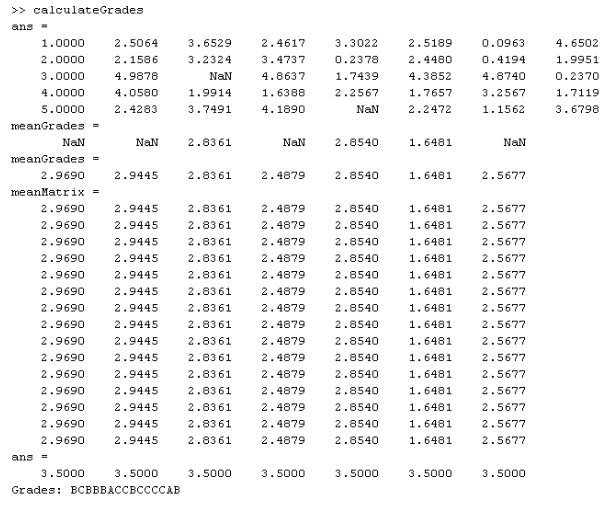
\includegraphics[width=\maxwidth{61.6156547917712em}]{imgCalculteGrades}

	\matlabheadingtwo{7. Gráficas}
	
	
	
	Abre un nuevo script y guárdalo como leyMoore.m\texttt{ }y resuelva el problema siguiente: \\
	
	
	De acuerdo con la ley de Moore (una observación hecha en 1965 por Gordon Moore, cofundador de Intel Corporation), el número de transistores que encajaría por pulgada cuadrada en un circuito integrado semiconductor se du- plica aproximadamente cada 18 meses. El año 2005 fue el 40 aniversario de la ley. Durante los últimos 40 años, su proyección se ha satisfecho de manera consistente. En 1965, la entonces tecnología de avanzada permitía 30 transistores por pulgada cuadra- da. La ley de Moore dice que la densidad de transistores se puede predecir mediante $d\left(t\right)=30\;\left(2^{\frac{t}{1\ldotp 5}} \right)$, donde $t$ se mide en años.
	
	
	
	
	\begin{enumerate}
		\item Sea $t=0$ la representación del año 1965 y $t=45$ la representación de 2010. Use este modelo para calcular el número predicho de transistores por pulgada cuadrada para los 45 años desde 1965 hasta 2010. Sea $t$ el aumento en incrementos de 1.5 años. Muestre los resultados en una tabla con 2 columnas, una para el año y otra para el número de transistores.
		
		\item Con la característica subplot, grafique los datos en una gráfica lineal x-y, una gráfica x semilog, una gráfica y semilog y una gráfica log-log. Asegúrese de poner título y etiqueta a los ejes.
		
		\item Guarde la figura como archivo 'ley\_moore.pdf'. Pero primero use el comando 'orient tall' para decirle a MATLAB que la figura llene la página impresa. Enumera los comandos que has utilizado a continuación.
	\end{enumerate}
	
	\vspace{1em}
	
	
\end{document}
